% !TeX root = ../proyecto.tex

\chapter{Resultados y Análisis}\label{ch:resultados-y-analisis}
En este capítulo se exponen los experimentos realizados y los resultados obtenidos en los distintos escenarios evaluados.
El objetivo principal fue analizar el rendimiento de los modelos entrenados con conjuntos de datos reducidos,
seleccionados mediante algoritmos meméticos y evolutivos.


\section{Resultados con el conjunto completo}\label{sec:resultados-conjunto-completo}
Como punto de partida, se evalua el rendimiento de los modelos convolucionales entrenados con el 100\% del conjunto de datos.
Esta prueba sirve como referencia para contrastar los resultados obtenidos mediante las técnicas de reducción aplicadas posteriormente.
Se utilizan tanto ResNet50 como MobileNetV2, y se miden métricas como accuracy, precisión, recall y F1-score sobre el conjunto de validación.

\begin{table}[htp]
    \centering
    \resizebox{\textwidth}{!}{
        \begin{tabular}{P{2cm} P{2.5cm} P{2.5cm} P{2.5cm} P{2cm} P{2cm} P{2cm} P{2cm}}
            \toprule
            \textbf{Duración Inferencia} & \textbf{Accuracy (Avg)} & \textbf{Precision (Avg)} & \textbf{Recall (Avg)} & \textbf{F1-score (Avg)} \\
            \midrule
            \multicolumn{8}{l}{\textbf{Modelo ResNet50}}                                                                                        \\
            \midrule
            00:02:42                     & 87,90\%                 & 88,96\%                  & 87,90\%               & 87,81\%                 \\
            \midrule
            \multicolumn{8}{l}{\textbf{Modelo MobileNet}}                                                                                       \\
            \midrule
            00:03:16                     & 78,60\%                 & 81,55\%                  & 78,60\%               & 77,68\%                 \\
            \bottomrule
        \end{tabular}
    }
    \caption{Comparativa de resultados del \textbf{100\%} con los modelos \textbf{ResNet50} y \textbf{MobileNet}.}
    \label{tab:resultados-100-resnet50-mobilenet}
\end{table}

Los resultados en la tabla~\ref{tab:resultados-100-resnet50} obtenidos representan el rendimiento máximo alcanzable en condiciones ideales,
sin reducción de datos, lo que permite establecer un techo de rendimiento frente al cual comparar las demás técnicas.


\section{Comparativa inicial de modelos}\label{sec:comparativa-inicial-modelos}
Antes de aplicar los algoritmos propuestos de reducción de datos, se considera fundamental realizar una comparativa inicial entre distintos
modelos de redes neuronales convolucionales para determinar cuál de ellos es el más adecuado para los experimentos.
Esta comparación permite identificar la arquitectura que ofrece un mejor equilibrio entre rendimiento y eficiencia computacional,
estableciendo una base sólida sobre la que construir los siguientes análisis.

Para llevar a cabo esta comparativa, se utiliza el \textbf{enfoque aleatorio} como estrategia de referencia.
Al seleccionar subconjuntos de datos de manera aleatoria, sin ninguna optimización, se obtiene una línea base que permiteº evaluar el
comportamiento de cada modelo en condiciones controladas.
Esta línea base es especialmente valiosa, ya que ofrece una perspectiva realista del rendimiento mínimo esperable sin aplicar técnicas
avanzadas de reducción de datos, sirviendo como punto de partida para comparar las mejoras introducidas por los algoritmos posteriores.


\begin{table}[htp]
    \centering
    \resizebox{\textwidth}{!}{
        \begin{tabular}{P{2cm} P{2.5cm} P{2.5cm} P{2.5cm} P{2cm} P{2cm} P{2cm} P{2cm}}
            \toprule
            \textbf{Porcentaje Inicial} & \textbf{Evaluaciones Realizadas} & \textbf{Duración Total} & \textbf{Duración Inferencia} &
            \textbf{Accuracy (Avg)}     & \textbf{Precision (Avg)}         & \textbf{Recall (Avg)}   & \textbf{F1-score (Avg)}                                              \\
            \midrule
            \multicolumn{8}{l}{\textbf{Modelo ResNet50}}                                                                                                                    \\
            \midrule
            10\%                        & 100                              & 00:45:08                & 00:00:27                     & 76,55\% & 81,80\% & 76,55\% & 76,25\% \\
            20\%                        & 100                              & 01:10:27                & 00:00:42                     & 81,77\% & 84,70\% & 81,77\% & 81,59\% \\
            50\%                        & 100                              & 02:24:49                & 00:01:26                     & 87,14\% & 88,09\% & 87,14\% & 86,97\% \\
            100\%                       & 1                                & -                       & 00:02:42                     & 87,90\% & 88,96\% & 87,90\% & 87,81\% \\
            \midrule
            \multicolumn{8}{l}{\textbf{Modelo MobileNet}}                                                                                                                   \\
            \midrule
            10\%                        & 100                              & 00:29:29                & 00:00:18                     & 72,31\% & 76,40\% & 72,31\% & 69,62\% \\
            20\%                        & 100                              & 00:50:36                & 00:00:30                     & 76,48\% & 78,82\% & 76,48\% & 75,58\% \\
            50\%                        & 100                              & 01:54:09                & 00:01:08                     & 75,56\% & 79,72\% & 75,56\% & 74,67\% \\
            100\%                       & 1                                & -                       & 00:03:16                     & 78,60\% & 81,55\% & 78,60\% & 77,68\% \\
            \bottomrule
        \end{tabular}
    }
    \caption{Comparativa de resultados de la generación inicial utilizando el algoritmo \textbf{aleatorio} y el \textbf{100\%} con los modelos \textbf{ResNet50} y \textbf{MobileNet}.}
    \label{tab:resnet50-vs-mobilenet}
\end{table}

\begin{figure}[htp]
    \centering
    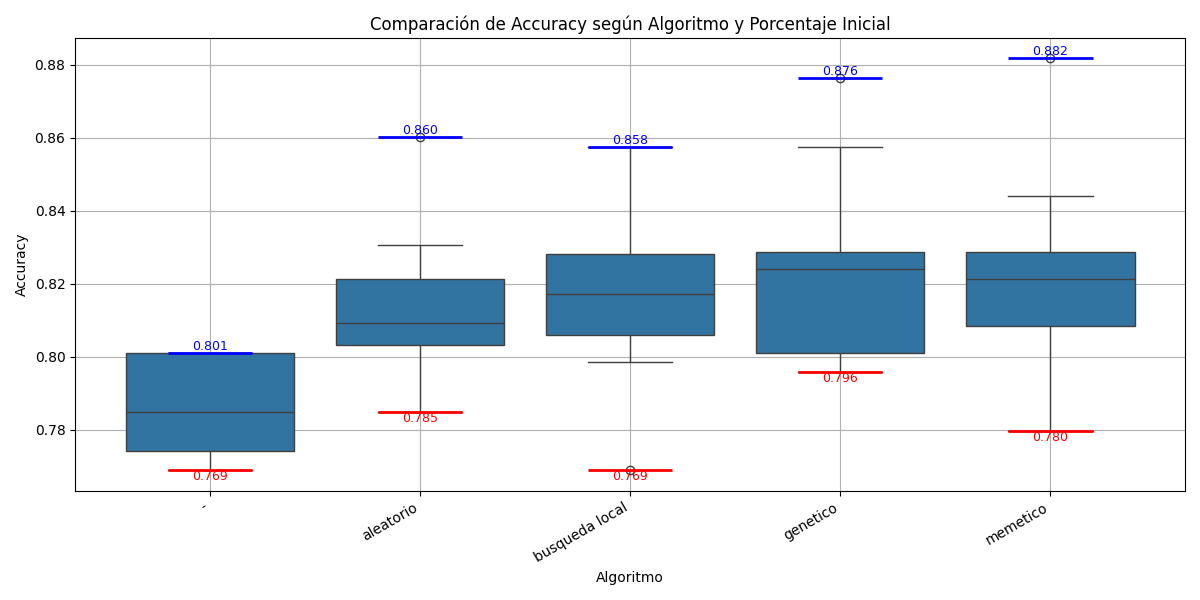
\includegraphics[width=0.95\textwidth]{imagenes/mobilenet-BOXPLOT-generacion-inicial}
    \caption{Boxplot comparando el \textit{accuracy} alcanzado por cada algoritmo de los iniciales.}
    \label{fig:resnet-boxplot-generacion-inicial}
\end{figure}

\colorbox{yellow}{Falta modificar la tabla~\ref{fig:resnet-boxplot-generacion-inicial} para que compare el 100\% con el aleatorio de resnet y ajustar analisis si es necesario.}
\colorbox{yellow}{Falta añadir tabla comparando resultados por porcentajes iniciales.}

Se realizan pruebas con distintos porcentajes iniciales de datos seleccionados aleatoriamente (10\%, 25\%, 50\%, 75\% y 100\%), utilizando tanto ResNet50 como MobileNetV2.
Los resultados obtenidos se presentan en la Tabla~\ref{tab:resnet50-vs-mobilenet}, que resume las métricas alcanzadas por cada modelo,
y en la Figura~\ref{fig:resnet-boxplot-generacion-inicial}, que muestra la distribución de los valores de \textit{accuracy} mediante boxplots.

Los resultados muestran que ResNet50 logra un mejor rendimiento en términos de \textit{accuracy}, \textit{precision}, \textit{recall} y \textit{F1-score}.
Sin embargo, este mejor rendimiento viene acompañado de un tiempo de entrenamiento considerablemente mayor.
Por su parte, MobileNetV2 ofrece una solución más eficiente en cuanto a tiempos de ejecución, a costa de una ligera pérdida de precisión,
lo que la convierte en una opción atractiva para entornos con recursos computacionales limitados.

En conjunto, esta comparativa inicial permite elegir MobileNetV2 como modelo principal para el resto de experimentos.
Aunque ResNet50 ofrece una precisión ligeramente superior, su elevado coste computacional no justifica su uso en las pruebas de reducción de datos,
donde la eficiencia es un factor clave.
Además, el uso del enfoque aleatorio como referencia permite establecer un punto de comparación para evaluar las mejoras que los algoritmos propuestos aportarían sobre esta línea base.


\section{Resultados de la búsqueda local}\label{sec:resultados-busqueda-local}
Como se describe en el apartado correspondiente (ver \hyperref[sec:algoritmo-busqueda-local]{Sección~\ref*{sec:algoritmo-busqueda-local}}),
la búsqueda local permite mejorar progresivamente una solución inicial mediante pequeñas modificaciones guiadas por el rendimiento.
En este apartado se evalúa su efectividad como alternativa más estructurada frente al enfoque aleatorio, pero sin llegar a la complejidad de los algoritmos evolutivos.
Su inclusión busca analizar hasta qué punto una estrategia simple pero guiada puede generar subconjuntos de datos más representativos y consistentes.

\begin{figure}[htp]
    \centering
    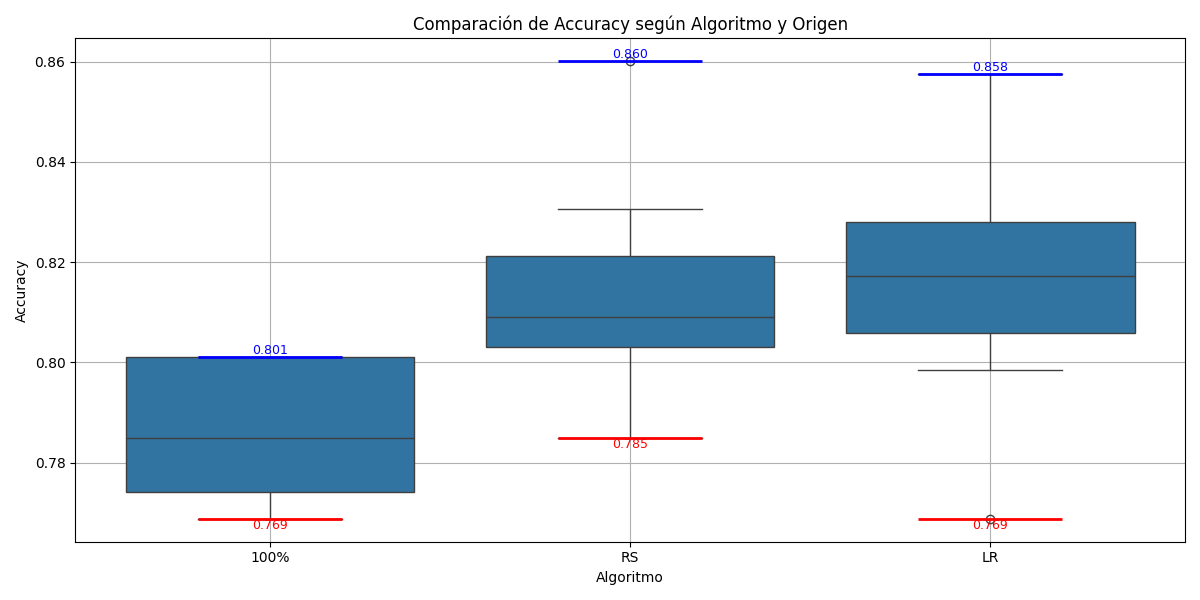
\includegraphics[width=1\textwidth]{imagenes/evaluaciones/comparacion_aleatorio-bl}
    \caption{Boxplot comparando el algoritmo aleatorio con la búsqueda local usando \textit{accuracy}.}
    \label{fig:aleatorio-vs-busqueda-local}
\end{figure}

En la Figura~\ref{fig:aleatorio-vs-busqueda-local} se muestran los resultados mediante un boxplot que permite observar
la distribución completa de valores obtenidos en las distintas ejecuciones.

Se puede apreciar que el algoritmo de búsqueda local mejora claramente la mediana del \textit{accuracy} respecto al enfoque aleatorio.
Mientras que el enfoque aleatorio se sitúa en torno a una mediana de 0.787, la búsqueda local alcanza una mediana superior, próxima a 0.818.
Esta diferencia refleja una mayor capacidad del algoritmo local para generar subconjuntos más representativos y eficaces.

Además, los valores máximos que alcanzan ambos algoritmos son similares (en torno a 0.858-0.860),
pero la búsqueda local muestra una dispersión más acotada hacia valores altos, lo que sugiere mayor estabilidad en sus resultados.
En cambio, el algoritmo aleatorio presenta una mayor dispersión hacia valores bajos y una mayor sensibilidad a la aleatoriedad de las selecciones,
como se evidencia en su menor valor mínimo (0.769 frente a 0.785 en búsqueda local).

Esto pone de manifiesto que, aunque el algoritmo aleatorio puede ocasionalmente alcanzar buenos resultados,
la búsqueda local ofrece una mejor consistencia y fiabilidad, con menos varianza entre ejecuciones y una tendencia general a obtener subconjuntos de entrenamiento más efectivos.


\section{Resultados del Algoritmo Genético}\label{sec:resultados-algoritmo-genetico}
Con el objetivo de superar las limitaciones observadas (como el riesgo de estancamiento o la exploración poco estructurada del espacio de soluciones)
se incorpora un enfoque evolutivo más completo: el algoritmo genético, descrito en la Sección~\ref{sec:genetico-v1}, el cual sirve como punto de partida para explorar la
aplicación de estrategias metaheurísticas en la selección de subconjuntos representativos de imágenes.
Su estructura evolutiva, basada en selección por torneo, cruce e incorporación de mutación,
ofrece ya desde sus primeras versiones una capacidad superior para generalizar, en comparación con métodos más simples como la búsqueda local.

\begin{figure}[htp]
    \centering
    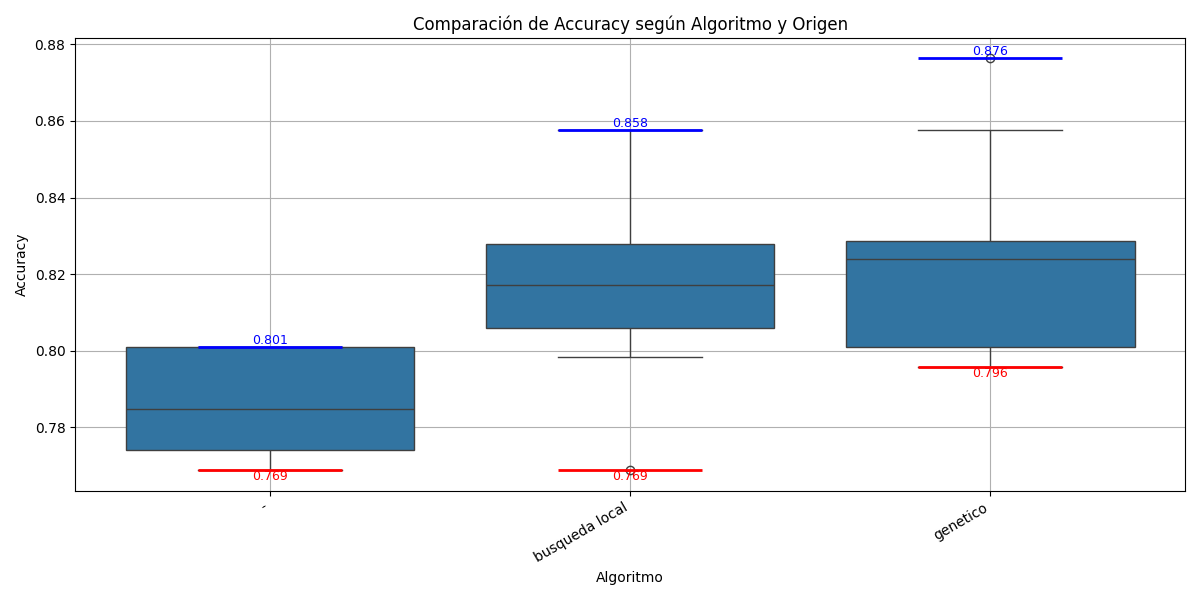
\includegraphics[width=1\textwidth]{imagenes/evaluaciones/comparacion_bl-gen_v1}
    \caption{Boxplot comparando la búsqueda local con el algoritmo genético v1 usando \textit{accuracy}.}
    \label{fig:bl-vs-gen-v1}
\end{figure}

Tal como se observa en la Figura~\ref{fig:bl-vs-gen-v1}, el algoritmo genético consigue una \textbf{mediana de \textit{accuracy}} más alta que la búsqueda local,
reflejando un rendimiento medio más consistente.
Además, presenta un valor máximo superior (alcanza hasta \textbf{0.876}), lo que evidencia su mayor potencial para encontrar soluciones de alta calidad.

No obstante, también se aprecia una ligera mayor dispersión en los resultados del algoritmo genético, particularmente hacia los valores bajos.
Esto indica que, pese a su capacidad exploratoria, el genético puede generar soluciones poco efectivas si no se controlan adecuadamente ciertos operadores como el cruce o la mutación.
De hecho, su valor mínimo (\textbf{0.796}) es superior al de la búsqueda local en esta comparativa,
pero deja margen para mejoras en la presión selectiva o en mecanismos que eviten estancamientos.

% \colorbox{yellow}{¿Sobra el siguiente apartado?}
La búsqueda local, por su parte, mantiene un comportamiento más estable, aunque con una mediana ligeramente inferior.
Su distribución es más concentrada y limitada en el extremo superior, lo que evidencia su carácter más explotador pero con menor capacidad para alcanzar soluciones óptimas globales.

Estos resultados sirven como evidencia empírica para continuar desarrollando nuevas versiones del algoritmo genético,
incorporando mejoras específicas en sus operadores con el fin de aprovechar su capacidad exploratoria y, al mismo tiempo, mitigar sus limitaciones.

\section{Mejorando el operador de cruce}\label{sec:incorporacion-cruce}
La primera mejora introducida al algoritmo genético consiste en reemplazar el cruce aleatorio por un cruce ponderado,
donde se prioriza la contribución del progenitor con mayor \textit{fitness}.
Además, se incorpora una estrategia selectiva que conserva únicamente el mejor de los dos hijos generados en cada cruce.
Ambos cambios, explicados en detalle en la \hyperref[sec:genetico-v2]{Sección~\ref*{sec:genetico-v2}},
buscan aumentar la presión evolutiva y acelerar la convergencia hacia soluciones de mayor calidad,
evitando así que soluciones mediocres se propaguen innecesariamente en la población.

\begin{figure}[htp]
    \centering
    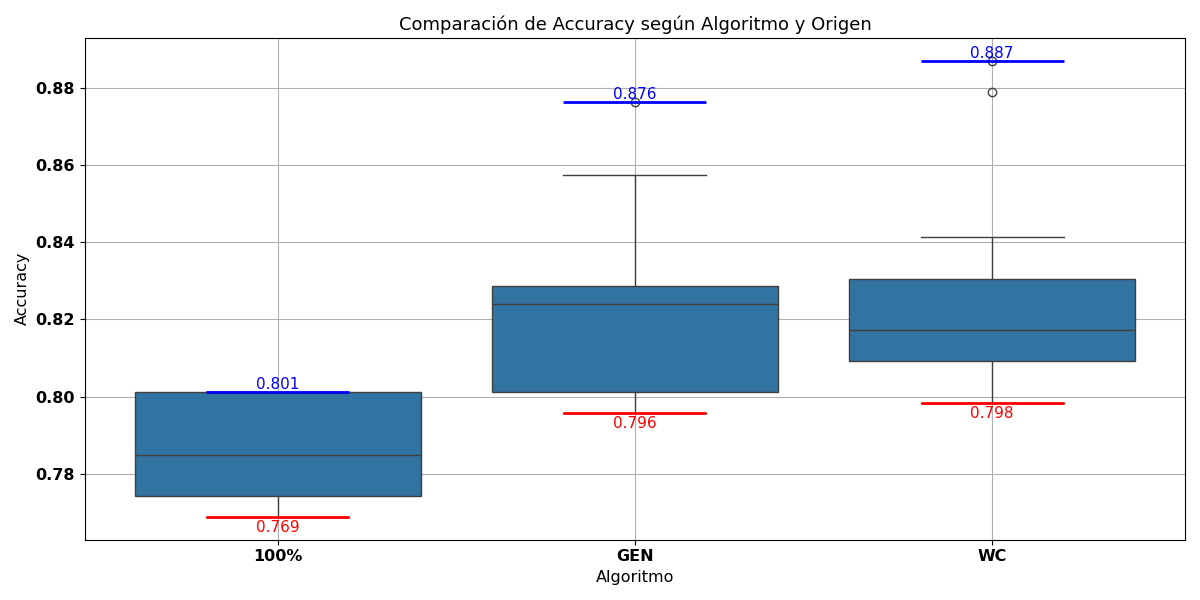
\includegraphics[width=1\textwidth]{imagenes/evaluaciones/operador-de-cruce}
    \caption{Boxplot de \textit{accuracy} para el genético, versión con cruce ponderado y dataset completo.}
    \label{fig:cruce_ponderado}
\end{figure}

Tal como se observa en la Figura~\ref{fig:cruce_ponderado}, esta modificación produce una mejora clara en la calidad y estabilidad de los resultados.
La versión con cruce ponderado (etiquetada como \texttt{genetico2}) alcanza un valor máximo atípico superior (\textbf{0.887}),
aunque presenta una mediana más baja que la versión básica.

Pero por otra parte, se aprecia una ligera reducción en la dispersión de los valores inferiores,
con un mínimo de \textbf{0.798} frente al \textbf{0.796} en la versión anterior, lo que sugiere una mayor consistencia.
Aunque el IQR (\hyperref[subsec:visualizacion-de-resultados]{Rango Intercuartílico}) sigue siendo amplio,
la acumulación de valores más cercanos al rango superior refleja una convergencia evolutiva más enfocada y menos dependiente del azar.

En conjunto, esta mejora en el cruce no solo permite una transferencia más eficiente de características ventajosas,
sino que también incrementa la presión selectiva sobre la calidad de las soluciones.
Esto se traduce en un comportamiento más robusto, menos propenso a resultados erráticos y con una mayor capacidad de exploración dirigida del espacio de soluciones.


\section{Mejorando el operador de mutación}\label{sec:mejorando-mutacion}
A partir de los resultados obtenidos con el algoritmo con cruce ponderado, se evalua una nueva versión en la que se introdujo una mutación adaptativa
(ver \hyperref[sec:genetico-mutacion]{Sección~\ref*{sec:genetico-mutacion}}).
A diferencia de la versión original con tasa fija, esta estrategia ajusta el número de intercambios en función del tamaño del subconjunto mutado,
lo que permite una mayor flexibilidad en escenarios de diferente escala.

\begin{figure}[htp]
    \centering
    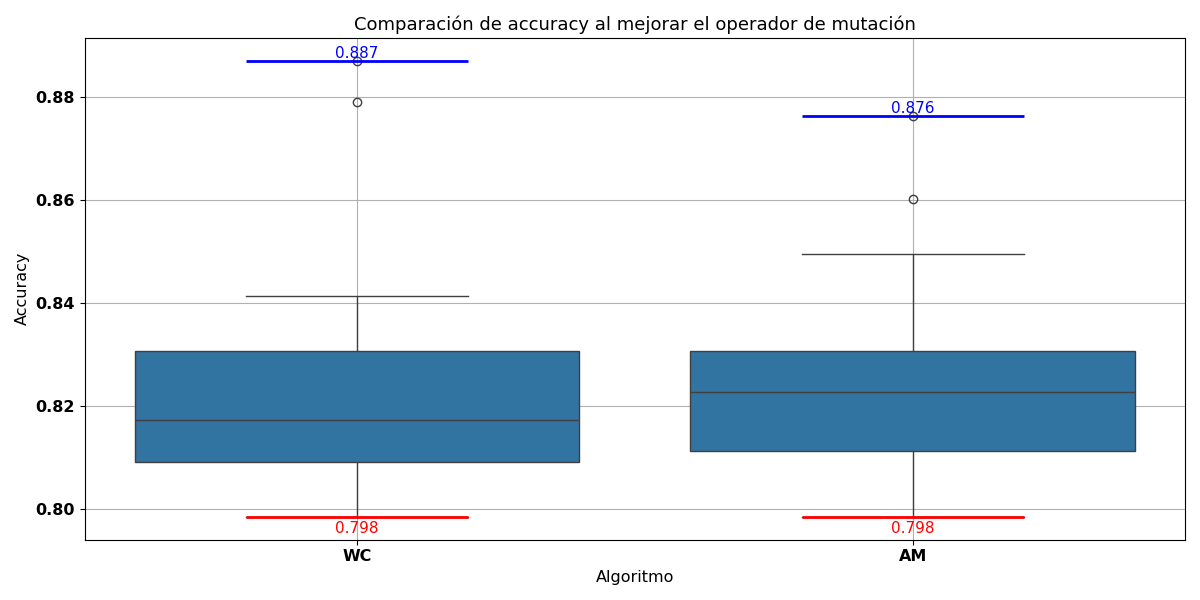
\includegraphics[width=1\textwidth]{imagenes/evaluaciones/mutacion-adaptativa}
    \caption{Comparación de \textit{accuracy} entre el algoritmo con cruce ponderado (\textit{genetico2}) y su versión con mutación adaptativa (\textit{genetico2\_2}).}
    \label{fig:mutacion-adaptativa}
\end{figure}

Como se observa en la Figura~\ref{fig:mutacion-adaptativa}, ambos algoritmos alcanzan un rendimiento similar en términos de mediana y valores extremos,
con una ligera ventaja de la versión original (\texttt{genetico2}) en el valor máximo de \textit{accuracy} (\textbf{0.887} frente a \textbf{0.876}).
Sin embargo, la versión con mutación adaptativa (\texttt{genetico2\_2}) muestra una distribución más compacta en la parte central,
con menos dispersión hacia valores bajos del IQR, lo que sugiere una mejora en la consistencia entre ejecuciones.

Además, la versión con mutación adaptativa presenta un Q4 más elevado, es decir, su \textit{bigote superior} abarca valores superiores a los de la versión original.
Esto indica que, aparte de que la mediana sea un poco superior, un mayor número de ejecuciones alcanzan rendimientos más altos de forma consistente,
reforzando la idea de que esta variante promueve una evolución más estable y con mayor concentración de soluciones de calidad en el tramo alto del rendimiento.

Este resultado refleja que, aunque la mutación adaptativa no produce una mejora radical en precisión media,
sí contribuye a una evolución más controlada y robusta, reduciendo la probabilidad de degradaciones abruptas.
Además, su comportamiento flexible la hace más adecuada en contextos donde el tamaño del subconjunto varía,
evitando configuraciones subóptimas impuestas por una tasa fija.

Aunque el valor máximo de \textit{accuracy} se mantiene en niveles similares, la ganancia está en la consistencia y la eficiencia exploratoria,
ya que se adapta automáticamente al contexto sin requerir ajustes manuales para diferentes tamaños de subconjuntos.
En conjunto, esta mejora refuerza la capacidad del algoritmo para mantener el equilibrio entre exploración y explotación durante el proceso evolutivo.


\section{Resultados del reinicio poblacional}\label{sec:resultados-reinicio-poblacional}
La Versión3 del algoritmo genético (ver \hyperref[sec:genetico-v3]{Sección~\ref*{sec:genetico-v3}})
introduce una lógica de reinicio poblacional diseñada para evitar estancamientos evolutivos.
El algoritmo monitoriza el rendimiento del segundo mejor individuo, y si este no mejora durante dos generaciones consecutivas,
se aplica un reinicio parcial que conserva únicamente al mejor individuo de la población.

\begin{figure}[htp]
    \centering
    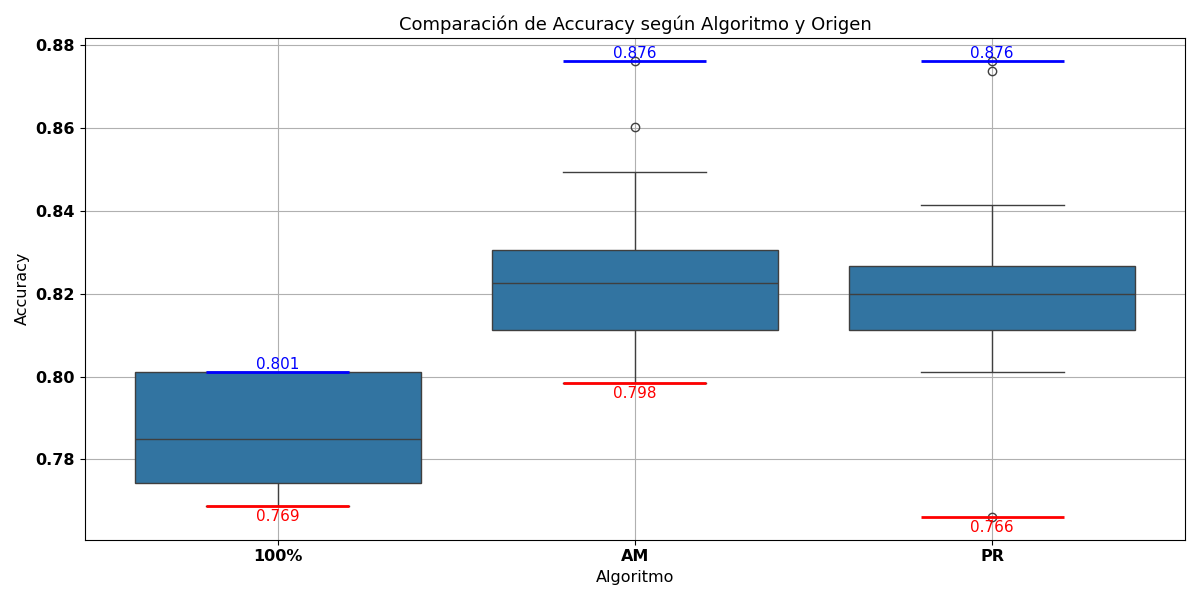
\includegraphics[width=1\textwidth]{imagenes/evaluaciones/reinicio-poblacional}
    \caption{Comparación de \textit{accuracy} entre el algoritmo genético con mutación adaptativa (genetico2\_2) y con reinicio poblacional (genetico3).}
    \label{fig:reinicio_poblacional}
\end{figure}

Tal como se observa en la Figura~\ref{fig:reinicio_poblacional}, los resultados muestran que la incorporación del reinicio no se traduce en una mejora tangible del rendimiento.
La mediana de \texttt{genetico3} permanece prácticamente inalterada respecto a \texttt{genetico2\_2} (incluso ligeramente inferior),
y aunque el valor mínimo es inferior (\textbf{0.766} frente a \textbf{0.798}), no se aprecia un incremento en el valor máximo ni una reducción clara en la dispersión.

Esto sugiere que, al menos en este contexto experimental, el mecanismo de reinicio no logra mejorar la exploración del espacio de soluciones
ni mitigar el estancamiento de forma eficaz.
En algunos casos, incluso puede introducir una pérdida prematura de diversidad, al regenerar de forma aleatoria parte de la población sin garantizar mejoras sustanciales.

% \colorbox{yellow}{¿Añadir el párrafo de resumen?}
% En resumen, aunque el reinicio poblacional es una estrategia teóricamente útil para escapar de óptimos locales,
% su implementación en esta versión no logró aportar beneficios consistentes en términos de rendimiento.
% Estos resultados invitan a reconsiderar su activación por defecto, o bien a explorar variantes más refinadas del mecanismo de reinicio.
En resumen, aunque el reinicio poblacional es una estrategia teóricamente útil para escapar de óptimos locales,
su implementación en esta versión no logra aportar beneficios consistentes en términos de rendimiento.

\section{Resultados con versiones libres}\label{sec:resultados-versiones-libres}
Como parte de la evolución de los algoritmos desarrollados, se proponen versiones libres,
en las que el tamaño del subconjunto seleccionado no permanece fijo durante la ejecución, sino que puede ajustarse de forma dinámica.

Para evaluar esta flexibilidad, se generan versiones libres de la búsqueda local y del algoritmo genético con cruce ponderado y mutación adaptativa,
como modificación adicional, se introduce un mecanismo al algoritmo de búsqueda local
en el que se selecciona de forma aletarioa el porcentaje inicial de imágenes a partir del cual se comienza a trabajar.


\begin{figure}[htp]
    \centering
    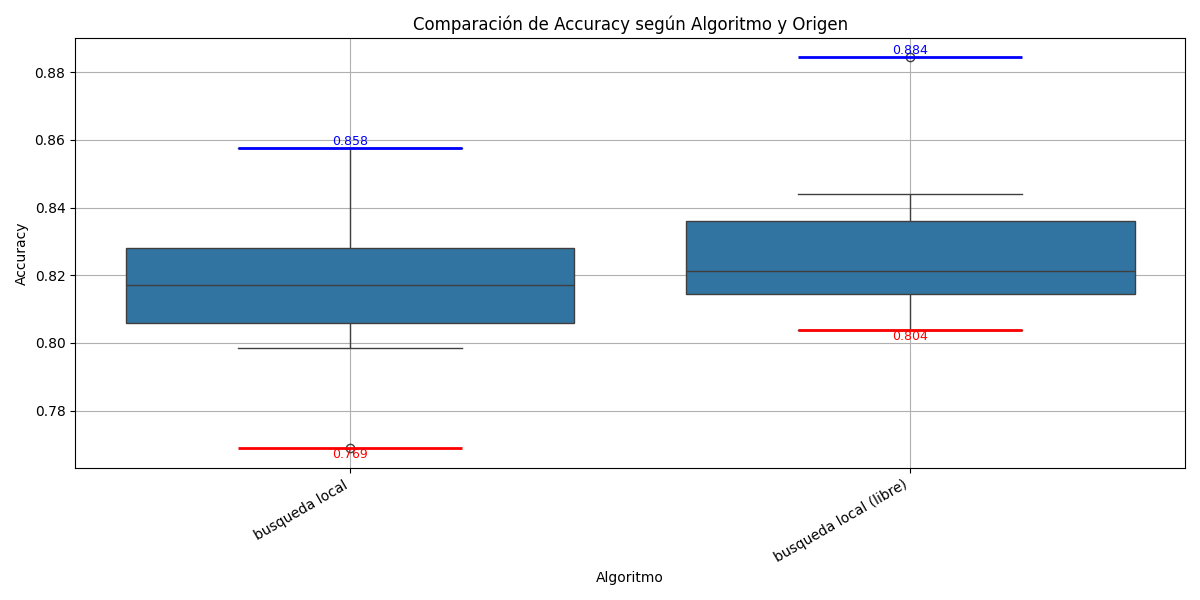
\includegraphics[width=0.9\textwidth]{imagenes/evaluaciones/libres/comparacion_bl}
    \caption{Comparación de \textit{accuracy} entre la búsqueda local estándar y su versión libre.}
    \label{fig:bl_libre}
\end{figure}

En la Figura~\ref{fig:bl_libre} se observa que la versión libre de la búsqueda local mejora tanto la mediana
como el valor máximo de \textit{accuracy} respecto a su versión original.
Presenta, además, una menor dispersión en los valores bajos y una mayor concentración de ejecuciones en torno al cuartil superior,
lo que sugiere una mejora en la estabilidad del algoritmo.
Este comportamiento refleja que introducir flexibilidad en el tamaño del subconjunto aporta capacidad de adaptación sin comprometer la consistencia del rendimiento.


\begin{figure}[htp]
    \centering
    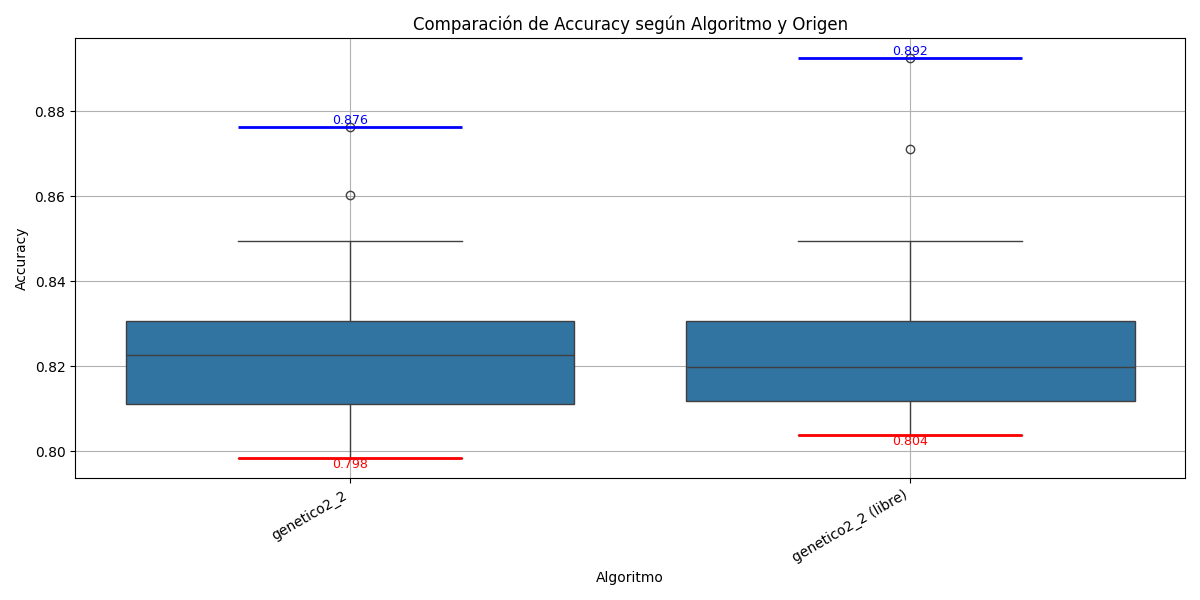
\includegraphics[width=0.9\textwidth]{imagenes/evaluaciones/libres/comparacion_gen_v2}
    \caption{Comparación de \textit{accuracy} entre el algoritmo genético v2-2 (cruce ponderado + mutación adaptativa) y su versión libre.}
    \label{fig:gen_v2_libre}
\end{figure}

En el caso del genético con cruce ponderado y mutación adaptativa (Figura~\ref{fig:gen_v2_libre}),
los resultados son algo más matizados: la versión libre mantiene un rendimiento muy similar al de la versión rígida,
con una leve mejora en los valores altos y un mínimo más elevado.
Esto sugiere que, aunque no siempre se observe una mejora significativa en mediana,
la capacidad adaptativa aporta robustez adicional y mayor protección frente a ejecuciones fallidas.


\colorbox{yellow}{Falta añadir boxplot que compare el accuracy separado por cada porcentaije inicail del algoritmo genetico 2 libre.}


\begin{figure}[htp]
    \centering
    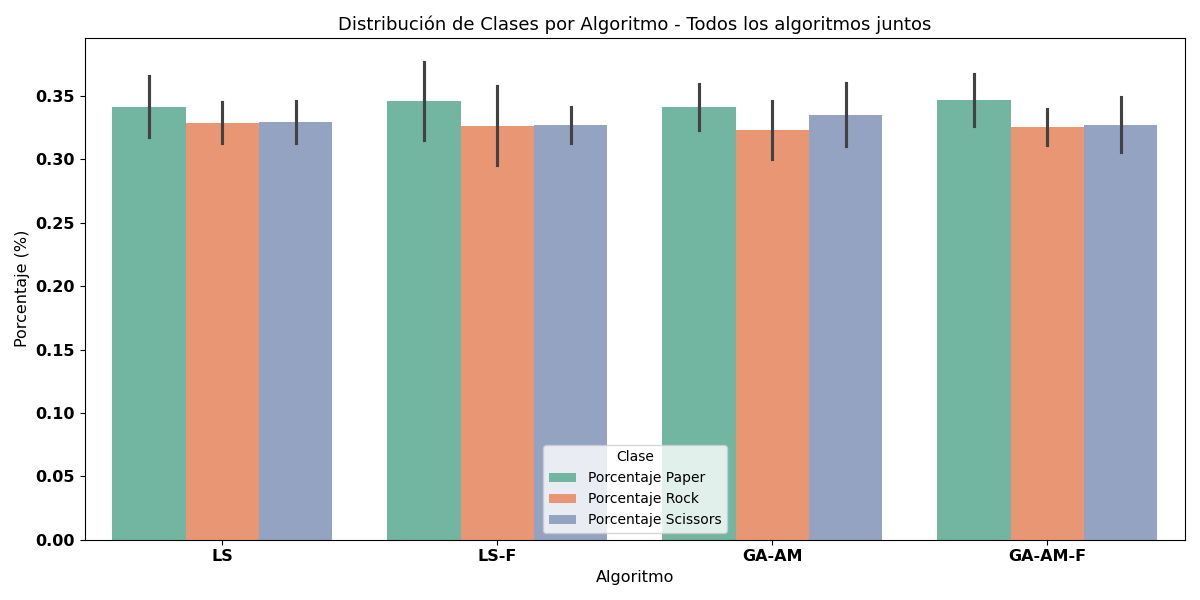
\includegraphics[width=0.9\textwidth]{imagenes/evaluaciones/libres/distribucion-clases}
    \caption{Distribución de clases en los subconjuntos generados por los algoritmos estándar y libres.}
    \label{fig:distribucion_libres}
\end{figure}

La Figura~\ref{fig:distribucion_libres} muestra que tanto los algoritmos estándar como sus variantes libres
mantienen una distribución equilibrada entre las tres clases del conjunto \texttt{RPS}.
Las proporciones de \texttt{Rock}, \texttt{Paper} y \texttt{Scissors} se reproducen de forma muy similar en todos los casos,
con únicamente pequeñas variaciones que no resultan significativas como para suponer un desbalance.

Este resultado es especialmente relevante para la validez de los experimentos, ya que confirma que los mecanismos evolutivos
y las estrategias de ajuste del tamaño del subconjunto no introducen sesgos de clase.
La representatividad estructural del conjunto se conserva, lo cual es fundamental para garantizar una evaluación justa y equilibrada en tareas de clasificación multiclase.


\begin{figure}[htp]
    \centering
    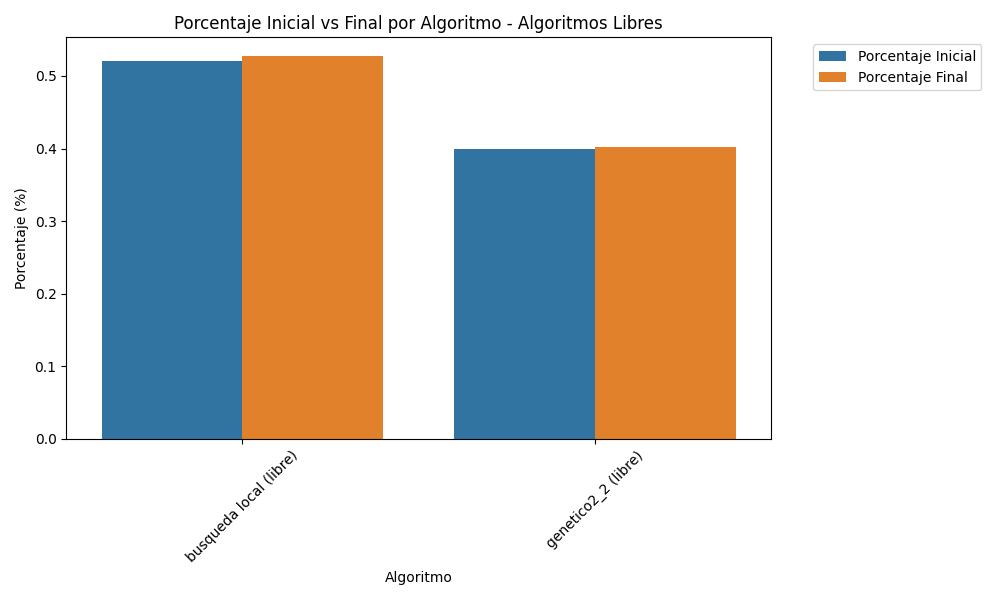
\includegraphics[width=0.9\textwidth]{imagenes/evaluaciones/libres/porcentaje-inical-vs-final-por-algoritmo}
    \caption{Comparación entre porcentaje inicial y final en los algoritmos libres.}
    \label{fig:porcentaje_libres_1}
\end{figure}

\begin{figure}[htp]
    \centering
    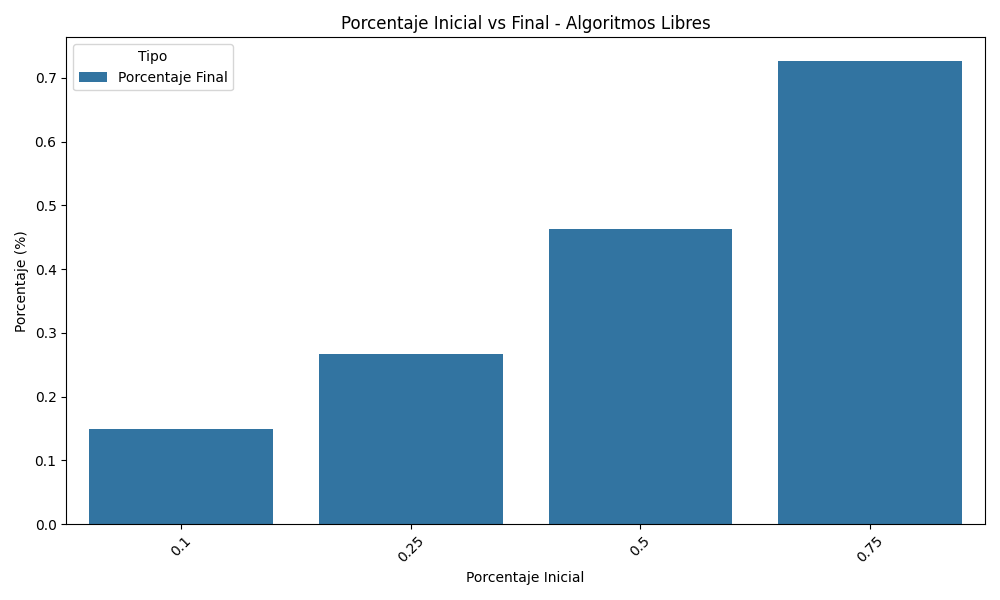
\includegraphics[width=0.9\textwidth]{imagenes/evaluaciones/libres/porcentaje-inicial-vs-final-por-pi_gev_v2.png}
    \vspace{1em}
    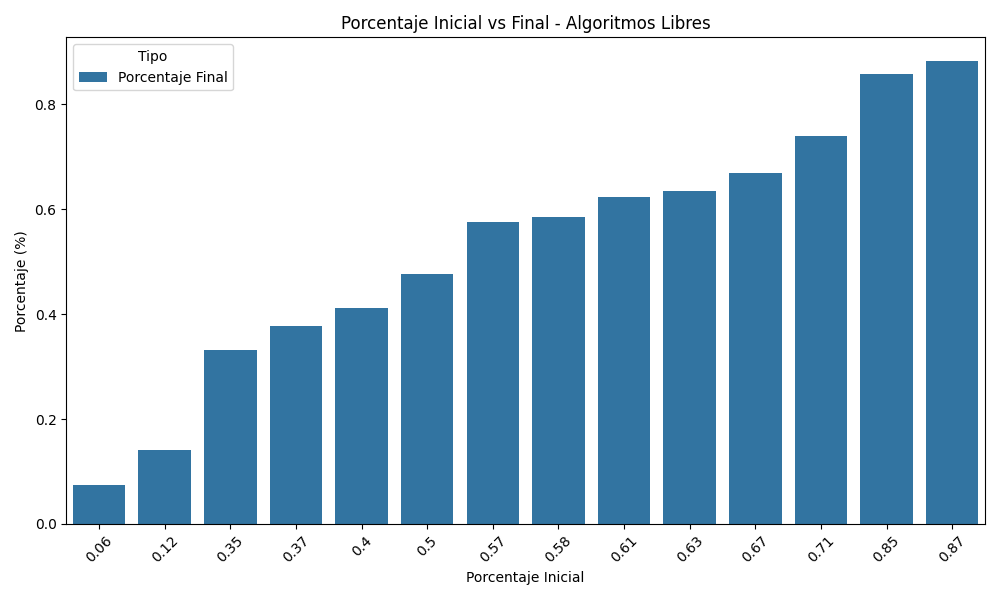
\includegraphics[width=0.9\textwidth]{imagenes/evaluaciones/libres/porcentaje-inicial-vs-final-por-pi_bl.png}
    \caption{Porcentaje final alcanzado en función del porcentaje inicial.
        Arriba: genético libre.
        Abajo: búsqueda local libre.
    }
    \label{fig:porcentaje_libres_2}
\end{figure}

Las Figuras~\ref{fig:porcentaje_libres_1} y~\ref{fig:porcentaje_libres_2} permiten analizar con mayor detalle cómo se comportan
los algoritmos libres en términos de tamaño del subconjunto seleccionado.
En la comparación directa por algoritmo (Figura~\ref{fig:porcentaje_libres_1}), se observa que el porcentaje final tiene un leve incremento respecto al inicial.

Sin embargo, al desglosar el análisis por valores específicos del porcentaje inicial (Figura~\ref{fig:porcentaje_libres_2}),
se aprecia un patrón más claro: cuanto mayor es el punto de partida, mayor tiende a ser también el porcentaje final alcanzado.
Esta tendencia es especialmente marcada en el caso de la búsqueda local libre, que muestra una progresión prácticamente lineal.
El algoritmo genético, en cambio, presenta un crecimiento más escalonado, pero igualmente adaptativo.

Este comportamiento sugiere que los algoritmos libres no solo adaptan la composición del subconjunto, sino también su escala,
ajustando dinámicamente la cantidad de datos seleccionados según el entorno de búsqueda.
En general, estas versiones demuestran ser una opción más versátil y controlada, especialmente útil cuando no se conoce de antemano el tamaño óptimo del conjunto de entrenamiento.


\section{Resultados del algoritmo memético}\label{sec:resultados-algoritmo-memetico}
Finalmente, se evalua el algoritmo memético (ver \hyperref[sec:algoritmo-memetico]{Sección~\ref*{sec:algoritmo-memetico}}),
el cual combina la evolución genética con una búsqueda local aplicada de forma probabilística sobre ciertos individuos seleccionados.
Este enfoque híbrido busca equilibrar la exploración del espacio de soluciones con una intensificación localizada,
ofreciendo mejoras tanto en precisión como en estabilidad.


\begin{figure}[htp]
    \centering
    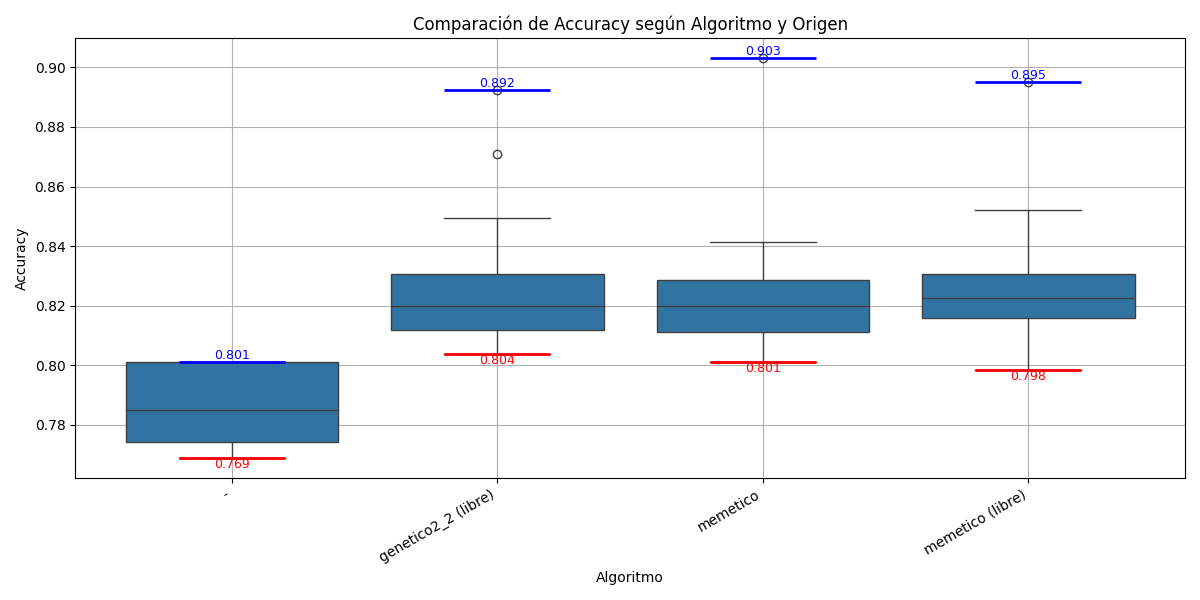
\includegraphics[width=0.9\textwidth]{imagenes/evaluaciones/comparacion-memetico}
    \caption{Comparación de \textit{accuracy} entre el algoritmo memético estándar y su versión libre.}
    \label{fig:memetico_comparacion}
\end{figure}

Tal como se aprecia en la Figura~\ref{fig:memetico_comparacion}, el algoritmo memético supera claramente al mejor de los enfoques genéticos
(el Genetico Libre con Cruce Ponderado y Mutación Adaptativa), alcanzando una mediana más elevada y un valor máximo de \textit{accuracy} de hasta \textbf{0.903}.
Su distribución es más compacta, con menor dispersión hacia los valores bajos, lo que refleja una mayor consistencia entre ejecuciones.

La versión libre del memético, que incorpora también un ajuste dinámico del tamaño del subconjunto
(ver \hyperref[subsec:memetico-libre]{Apartado~\ref*{subsec:memetico-libre}}), muestra un rendimiento muy similar al estándar,
con una ligera reducción en el valor máximo pero una estabilidad comparable.
Esto sugiere que el componente adaptativo no penaliza la calidad de las soluciones y puede incluso aportar mayor flexibilidad en entornos más inciertos.

\begin{figure}[htp]
    \centering
    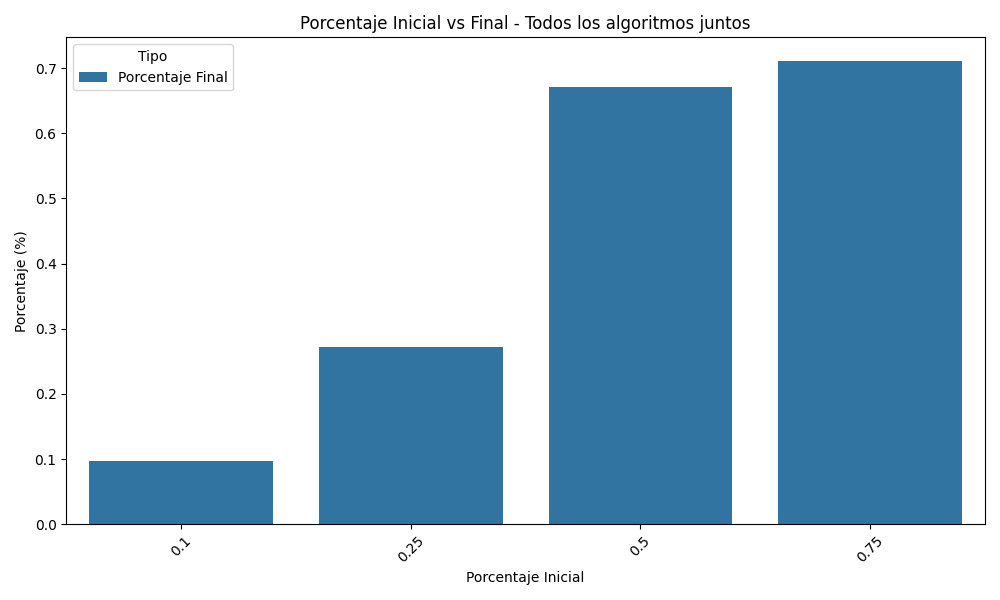
\includegraphics[width=0.9\textwidth]{imagenes/evaluaciones/libres/porcentaje-inicial-vs-final-por-pi_memetico-libre}
    \caption{Porcentaje final alcanzado por el algoritmo memético libre en función del porcentaje inicial.}
    \label{fig:memetico_porcentaje}
\end{figure}

En la Figura~\ref{fig:memetico_porcentaje} se observa cómo el memético libre tiende a incrementar el tamaño del subconjunto conforme aumenta el porcentaje inicial.
La curva es progresiva y cercana a la linealidad, lo que indica un comportamiento estructuralmente coherente:
el algoritmo detecta cuándo puede beneficiarse de incluir más ejemplos y adapta su escala en consecuencia.
Este ajuste dinámico refuerza su capacidad para equilibrar rendimiento y tamaño, maximizando la eficiencia de la selección sin depender de una configuración fija.

% \colorbox{yellow}{¿Añadir el párrafo de resumen?}
De esta forma, tanto el memético estándar como su variante libre se consolidan como las estrategias más eficaces del estudio.
% Su combinación de precisión elevada, estabilidad entre ejecuciones y capacidad adaptativa los convierte en soluciones
% especialmente robustas para tareas donde se requiere seleccionar subconjuntos representativos sin comprometer el rendimiento del modelo entrenado.


\section{Resultados finales entre enfoques}\label{sec:comparacion-final-enfoques}
En esta sección se realiza una comparación conjunta entre todos los algoritmos implementados.
Se presentan boxplots y gráficos de barras que muestran la evolución del \textit{accuracy}, el porcentaje de datos utilizados y el equilibrio entre clases.

% Los algoritmos meméticos y genéticos v2/v3 (especialmente en sus versiones libres) destacan como los más eficaces, consiguiendo una reducción significativa del conjunto de entrenamiento sin penalizar la precisión.
% Además, se observa una menor varianza en sus resultados, lo que indica una mayor consistencia entre ejecuciones.

\colorbox{yellow}{Falta realizar la comparación final.}


\section{Validación con el dataset \texttt{PAINTING}}\label{sec:validacion-con-painting}
Para comprobar la robustez de los algoritmos desarrollados, se validan los experimentos con el dataset \texttt{PAINTING},
caracterizado por una mayor complejidad visual y un número superior de clases respecto al conjunto \texttt{RPS}.
Con el fin de mantener un equilibrio entre complejidad y coste computacional, se limitan los experimentos a los porcentajes iniciales del 25\% y 50\%,
evaluando únicamente los algoritmos más representativos.

En particular, se selecciona el algoritmo memético, junto con su versión libre, ya que ambos han demostrado ser los más eficaces en las pruebas anteriores.
Para establecer una referencia clara, se incluyen también los resultados obtenidos usando el 100\% del conjunto de datos, y para la comparación de
\textit{accuracy} entre algoritmos también se añade el resultado del algoritmo aleatorio.

\subsection{Comparación de \textit{accuracy} entre algoritmos}
\begin{figure}[htp]
    \centering
    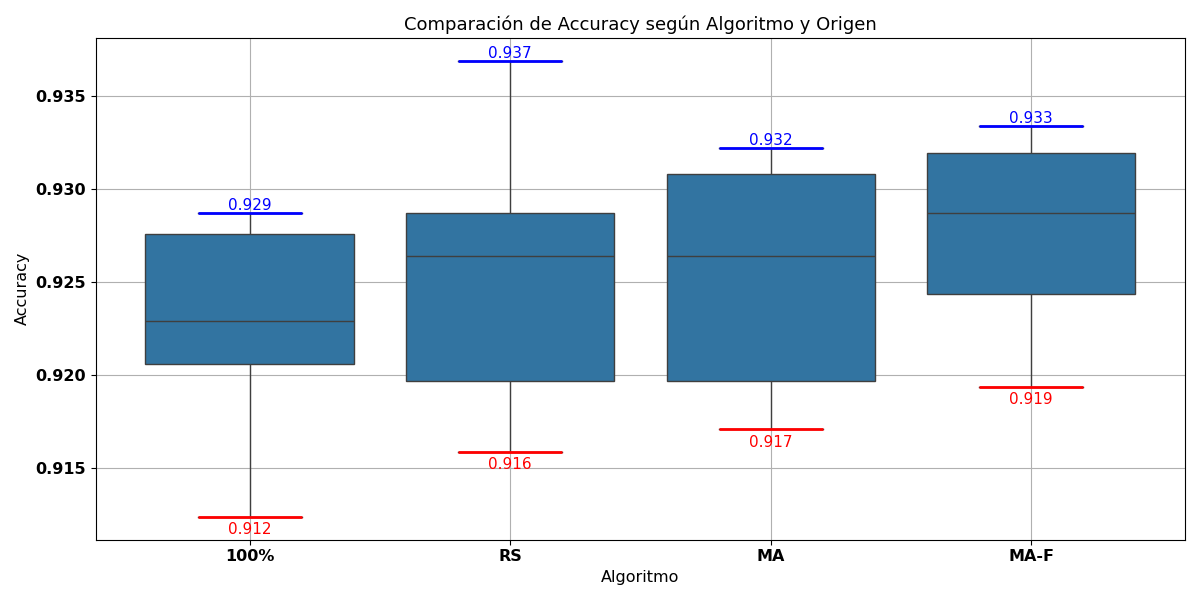
\includegraphics[width=1\textwidth]{imagenes/evaluaciones/painting/comparacion-por-algoritmo}
    \caption{Boxplot comparando resultados con el dataset \texttt{PAINTING} usando \textit{accuracy}.}
    \label{fig:comparacion-por-algoritmo}
\end{figure}

En la Figura~\ref{fig:comparacion-por-algoritmo} se comparan los valores de \textit{accuracy} obtenidos al aplicar distintos
algoritmos de selección de subconjuntos en el conjunto de datos \texttt{PAINTING}.
A simple vista, destaca el buen rendimiento de los tres enfoques meméticos frente al uso directo del 100\% del conjunto o la selección aleatoria,
lo cual es especialmente significativo al tratarse de un conjunto con alta complejidad visual y estructural.

El algoritmo memético libre obtiene el mejor rendimiento general, con una mediana que ronda el \textbf{0.927} y un valor máximo de \textbf{0.933},
superando incluso la ejecución con el 100\% de los datos, cuyo máximo se sitúa en \textbf{0.929}.
Esto no solo refuerza su capacidad de generalización, sino que demuestra que una selección optimizada puede superar a la totalidad del conjunto original,
posiblemente por eliminar ejemplos redundantes o incluso perjudiciales.

El algoritmo memético estándar también muestra una precisión elevada, con una mediana apenas inferior al libre, y un máximo de \textbf{0.931}.
Sin embargo, su varianza es ligeramente mayor, lo que sugiere que la falta de ajuste dinámico del tamaño del subconjunto puede limitar su adaptabilidad en ciertas ejecuciones.

Por otro lado, la selección aleatoria, aunque muestra valores aceptables, vuelve a confirmar su principal debilidad: la alta dispersión.
Con un mínimo de \textbf{0.916} y una mediana prácticamente idéntica a la obtenida con el uso completo del dataset,
su comportamiento se sitúa como una referencia básica pero poco fiable.
Puede alcanzar buenos resultados, pero lo hace de forma inconsistente y sin mecanismos que garanticen estabilidad.

La ejecución con el \textbf{100\%} de los datos, utilizada como referencia absoluta, queda por debajo de las soluciones obtenidas por los algoritmos meméticos.
Esto valida empíricamente que no es la cantidad de datos, sino su calidad y representatividad, lo que determina la eficacia del entrenamiento en entornos complejos.

% \colorbox{yellow}{¿Añadir el párrafo de resumen?}
% En conjunto, esta comparación deja clara la superioridad de las estrategias meméticas, especialmente en su versión libre,
% tanto por su rendimiento medio como por su estabilidad.
% Esto refuerza la hipótesis de que los algoritmos de selección basados en evolución y búsqueda local son capaces de generar
% subconjuntos más eficientes y fiables que los enfoques ingenuos o el uso total de los datos.
En resumen, los algoritmos meméticos, especialmente en su versión libre, muestran el mejor rendimiento en términos de precisión y estabilidad,
superando al uso del 100\% de los datos y al enfoque aleatorio.

\subsection{Impacto del porcentaje inicial}
\begin{figure}[htp]
    \centering
    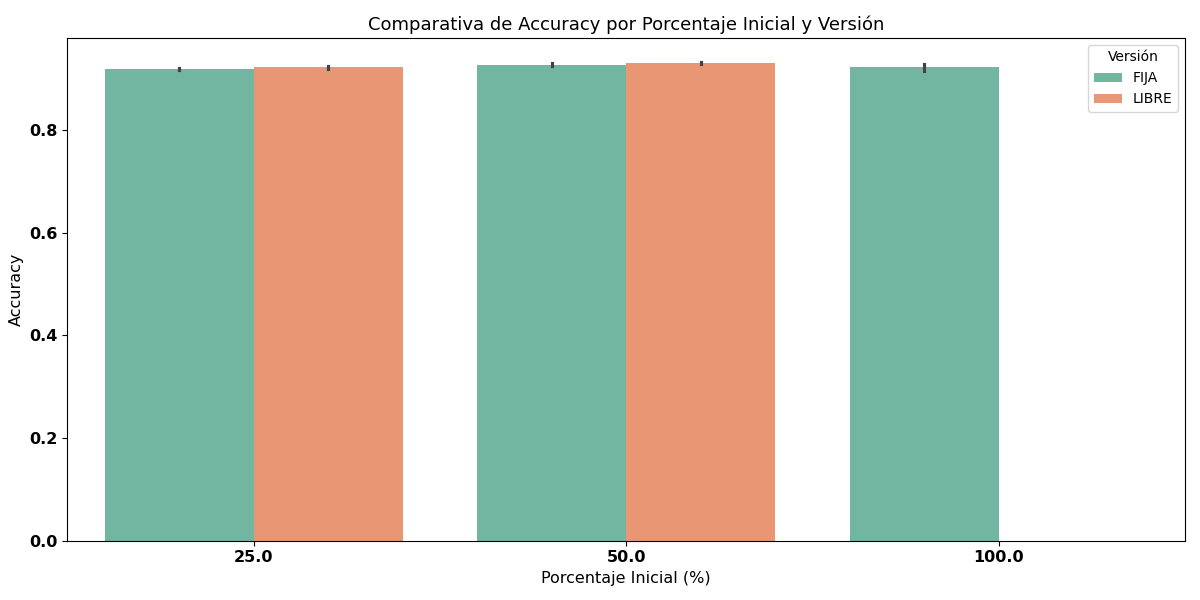
\includegraphics[width=1\textwidth]{imagenes/evaluaciones/painting/comparacion-por-porcentaje}
    \caption{Boxplot de \textit{accuracy} según el porcentaje inicial de datos.}
    \label{fig:accuracy_porcentaje_painting}
\end{figure}

La Figura~\ref{fig:accuracy_porcentaje_painting} muestra cómo varía el rendimiento del modelo (medido en términos de \textit{accuracy})
al utilizar diferentes porcentajes iniciales de datos para los algoritmos meméticos en el dataset \texttt{PAINTING}.
Lo primero que destaca es que el uso del 50\% del conjunto original no solo logra un rendimiento equiparable, sino incluso superior al uso del 100\%.
Con una mediana cercana a \textbf{0.930} y un máximo de \textbf{0.933}, este porcentaje logra un equilibrio ideal entre compresión de datos y preservación de información relevante.

Este resultado sugiere que, a partir de cierto umbral, añadir más datos no solo deja de aportar valor, sino que puede introducir ruido o redundancia.
En este caso, el entrenamiento con el 100\% de los datos exhibe mayor dispersión y un mínimo significativamente más bajo (\textbf{0.912}),
lo cual indica una mayor variabilidad entre ejecuciones y una menor estabilidad general.

Por otro lado, el uso del 25\% inicial también demuestra un rendimiento sorprendentemente competitivo,
alcanzando un máximo de \textbf{0.925}.
Sin embargo, su rango intercuartílico más estrecho (menor dispersión de los resultados) y su menor valor mínimo
(\textbf{0.917}) evidencian una cierta fragilidad ante la reducción excesiva:
puede funcionar bien si la selección es óptima, pero el margen de error es menor.

Este comportamiento ilustra un fenómeno interesante en la reducción de datos: no existe una relación lineal entre cantidad de datos y precisión,
sino que el valor está en la calidad y representatividad del subconjunto.
El resultado más robusto refuerza la hipótesis de que existe un punto de saturación
a partir del cual la adición de ejemplos tiene un efecto marginal o incluso contraproducente en modelos convolucionales.

% \colorbox{yellow}{¿Añadir el párrafo de resumen?}
% En conjunto, los resultados de este apartado respaldan la viabilidad de aplicar técnicas de reducción de datos en entornos reales,
% sugiriendo que con solo la mitad de los datos cuidadosamente seleccionados se puede no solo igualar,
% sino superar el rendimiento de un entrenamiento exhaustivo con todo el dataset.
En resumen, los resultados respaldan la viabilidad de utilizar una fracción cuidadosamente seleccionada de datos para obtener
resultados comparables o incluso superiores al uso del conjunto completo.

\subsection{Equilibrio en la distribución de clases}
\begin{figure}[htp]
    \centering
    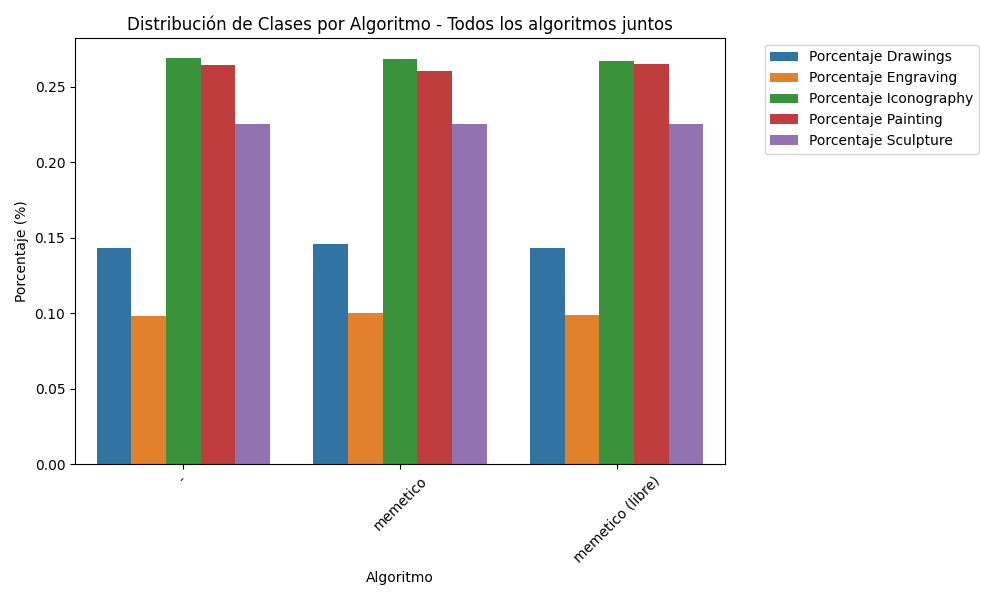
\includegraphics[width=0.9\textwidth]{imagenes/evaluaciones/painting/balance-de-clases-por-algoritmo}
    \caption{Distribución de clases seleccionadas por cada algoritmo.}
    \label{fig:balance_clases_painting}
\end{figure}

La Figura~\ref{fig:balance_clases_painting} muestra la proporción de clases preservada por cada algoritmo durante el proceso de reducción.
Se observa que tanto el algoritmo memético estándar como el libre mantienen una distribución prácticamente idéntica a la original,
sin introducir sesgos estructurales.

Las clases mayoritarias (\texttt{Iconography}, \texttt{Painting} y \texttt{Sculpture}) se mantienen consistentes en su proporción,
al igual que las clases minoritarias (\texttt{Drawings} y \texttt{Engraving}).
Esta conservación sugiere que el proceso de selección no actúa de forma aleatoria ni ciega,
sino que incorpora implícitamente una presión hacia la diversidad, lo cual es clave en problemas multiclase.

\subsection{Evolución del tamaño del subconjunto}
\begin{figure}[htp]
    \centering
    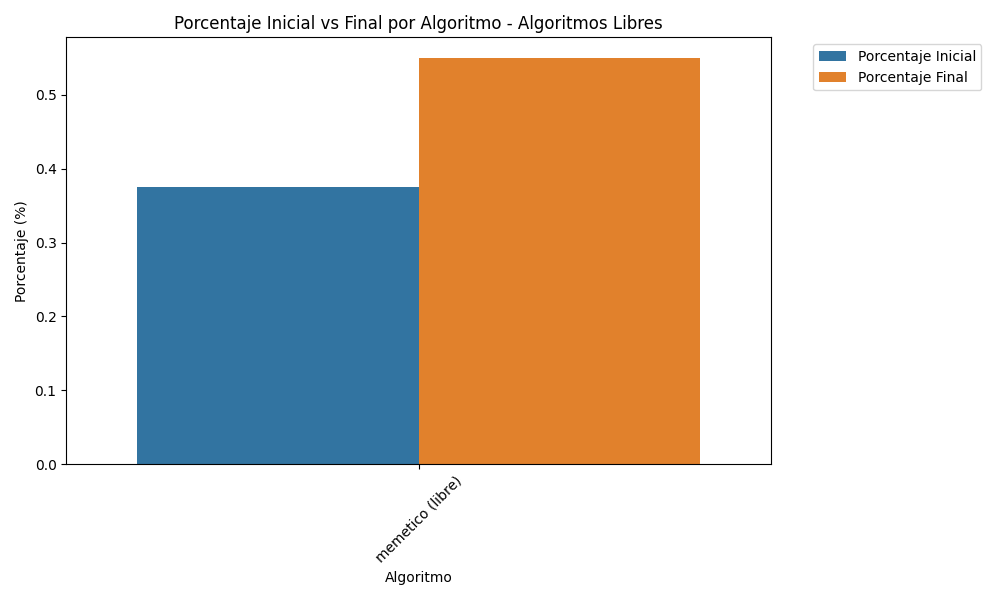
\includegraphics[width=0.9\textwidth]{imagenes/evaluaciones/painting/porcentaje-inical-vs-final-por-algoritmo}
    \vspace{1em}
    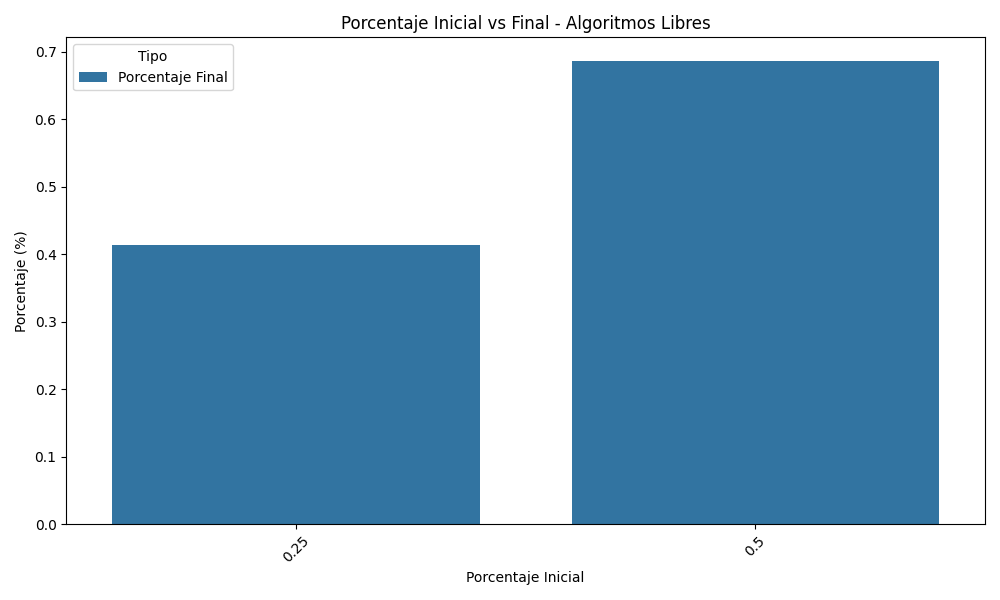
\includegraphics[width=0.9\textwidth]{imagenes/evaluaciones/painting/porcentaje-inicial-vs-final-por-pi}
    \caption{Evolución del tamaño del subconjunto seleccionado por los algoritmos libres.
        Arriba: comparación por algoritmo.
        Abajo: evolución según el porcentaje inicial.
    }
    \label{fig:evolucion_porcentaje_libre}
\end{figure}

En la Figura~\ref{fig:evolucion_porcentaje_libre} se analiza cómo evoluciona el tamaño de los subconjuntos seleccionados por los algoritmos libres respecto al valor inicial.
Se observa que el algoritmo memético libre tiende a incrementar el porcentaje de imágenes seleccionadas durante el proceso evolutivo.

Este comportamiento adaptativo pone de manifiesto la capacidad del algoritmo para ajustar dinámicamente la escala de la solución en función de la complejidad del problema.
A diferencia de enfoques con tamaño fijo, el algoritmo libre no solo decide qué ejemplos seleccionar, sino también cuántos,
ampliando el conjunto cuando detecta que puede mejorar el rendimiento sin incurrir en sobreajuste.

Además, se observa que al partir del 25\% inicial, el algoritmo tiende a aumentar el tamaño del subconjunto hasta un 16,35\% adicional,
en cambio, al partir del 50\% inicial, el crecimiento es mayor, alcanzando un 18,69\% adicional~\footnote{Porcentajes exactos sacados de la tabla de resultados.}.
Este hecho puede sugerir una cierta prudencia evolutiva: el algoritmo no se expande indiscriminadamente,
sino que responde a señales de mejora en el proceso de evaluación.
Este mecanismo emergente refuerza la versatilidad del enfoque libre, que no solo busca soluciones de alta calidad,
sino que lo hace optimizando también el volumen de datos utilizados.


\bigskip

\subsection*{Síntesis final de la validación con \texttt{PAINTING}}
Los resultados obtenidos con el dataset \texttt{PAINTING} confirman la solidez y capacidad de generalización de los algoritmos desarrollados.
Tanto el enfoque memético estándar como, especialmente, su versión libre, lograron mantener un rendimiento competitivo en un entorno más complejo y con mayor número de clases.

Se evidencia que es posible superar el rendimiento del conjunto completo de entrenamiento utilizando únicamente un subconjunto bien seleccionado,
reduciendo significativamente el volumen de datos sin comprometer la precisión.
Además, los algoritmos meméticos demuestra preservar el equilibrio entre clases y adaptarse dinámicamente al tamaño del subconjunto,
lo que constituye una ventaja clave en tareas reales donde no siempre se dispone de datasets perfectamente balanceados ni completos.

En conjunto, esta validación externa no solo refuerza las conclusiones obtenidas con \texttt{RPS},
sino que demuestra que el uso de técnicas evolutivas, y en particular las variantes libres, puede ser una alternativa eficaz,
escalable y controlable frente a la selección masiva o aleatoria de datos en procesos de entrenamiento profundo.
